\documentclass[usenames,dvipsnames]{beamer}
\usepackage[utf8]{inputenc}
\usepackage[T1]{fontenc}
\usepackage[french]{babel}
\usepackage{xcolor}
\usepackage{pifont}
\usetheme{Singapore} %Boadilla | Bergen | Madrid | Antibes | Hannover | Singapore | Warsaw

\newcommand{\cmark}{\ding{51}}
\newcommand{\xmark}{\ding{55}}
%----------------------------------------------------------------------------------------
%   TITLE INFORMATION
%----------------------------------------------------------------------------------------
\title{Entrepôts de données pour \textit{Tam voyages}}
\subtitle{HMIN122M -- Entrepôts de Données et Big-Data}
\author{B. Rima \and J. Saba \and T. Shaqura \and J. Bourgin}
\institute[UM]{M1 Informatique AIGLE}
\date{\today}

\begin{document}
%----------------------------------------------------------------------------------------
%   TITLE FRAME
%----------------------------------------------------------------------------------------
\begin{frame}
\titlepage
\end{frame}
%----------------------------------------------------------------------------------------
%   OUTLINE
%----------------------------------------------------------------------------------------
\begin{frame}{Sommaire}
\tableofcontents
\end{frame}
%----------------------------------------------------------------------------------------
%   INTRODUCTION
%----------------------------------------------------------------------------------------
\section{Introduction}
\begin{frame}{Contexte du projet}{Introduction}
\end{frame}

\section{Modélisation}
\begin{frame}{Contexte du projet}{Introduction}
\end{frame}

\section{Implémentation}
\begin{frame}{Implémentation}{Quel choix faire ?}
\begin{figure}[!ht]
  \centering
  
\includegraphics[scale=0.5]{images/Oracle.png}
  \caption{Oracle, What else ?}
\end{figure}
\end{frame}

\subsection{le nombre de voyage par bus, utilisant des tickets pour le mois de juillet}
\begin{frame}{Implémentation}{le nombre de voyage par bus, utilisant des tickets pour le mois de juillet}
\begin{figure}[!ht]
  \centering
  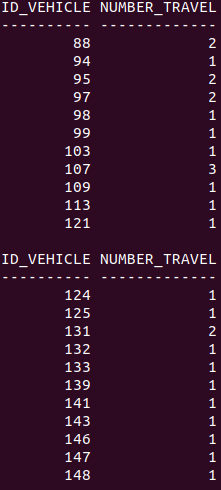
\includegraphics[scale=0.5]{images/requetes_analytiques/requ1.png}
\end{figure}
\end{frame}

\subsection{le nombre de voyageurs abonnés par ligne pour chaque voyage pour les deux derniers mois}
\begin{frame}{Implémentation}{le nombre de voyageurs abonnés par ligne pour chaque voyage pour les deux derniers mois}
\begin{figure}[!ht]
  \centering
  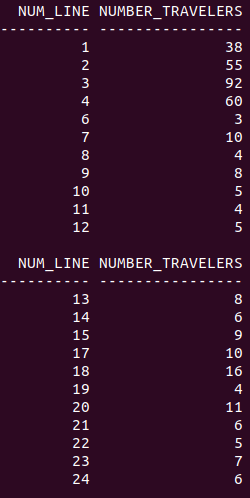
\includegraphics[scale=0.5]{images/requetes_analytiques/requ2.png}
\end{figure}
\end{frame}

\subsection{l'arrêt le plus fréquenté par ligne}
\begin{frame}{Implémentation}{l'arrêt le plus fréquenté par ligne}
\begin{figure}[!ht]
  \centering
  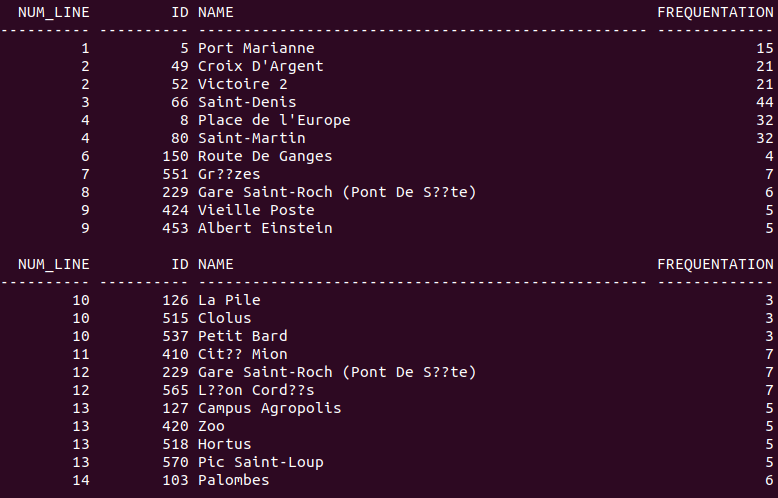
\includegraphics[scale=0.5]{images/requetes_analytiques/requ3.png}
\end{figure}
\end{frame}

\subsection{le coût total de maintenance de chaque véhicule}
\begin{frame}{Implémentation}{le coût total de maintenance de chaque véhicule}
\begin{figure}[!ht]
  \centering
  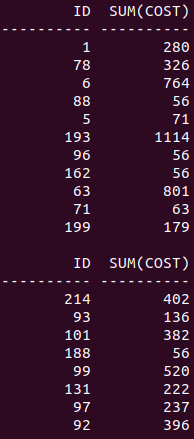
\includegraphics[scale=0.5]{images/requetes_analytiques/requ6.png}
\end{figure}
\end{frame}

\subsection{le nombre total de maintenances effectuées sur les bus par employé pour l'année 2018}
\begin{frame}{Implémentation}{le nombre total de maintenances effectuées sur les bus par employé pour l'année 2018}
\begin{figure}[!ht]
  \centering
  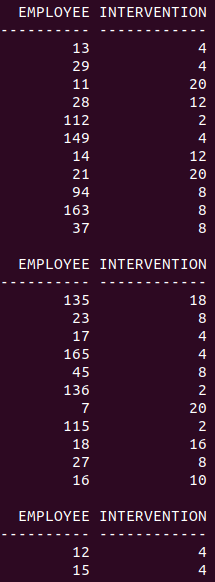
\includegraphics[scale=0.5]{images/requetes_analytiques/requ7.png}
\end{figure}
\end{frame}

\section{Conclusion}
\begin{frame}{Contexte du projet}{Introduction}
\end{frame}
\end{document}
